% !TEX program = xelatex
% !LW recipe = XeLaTeX
% OpenDyslexic version for easier manual review.
% Compile with: xelatex Redefining_Racism_OpenDyslexic.tex
% (OpenDyslexic font must be installed: https://opendyslexic.org/)

\documentclass[12pt]{article}

\usepackage{fontspec}
\setmainfont{OpenDyslexic3}

\usepackage{microtype}
\usepackage{amsmath,amssymb}
\usepackage{geometry}
\usepackage[colorlinks=true, linkcolor=black, citecolor=black, urlcolor=blue]{hyperref}
\usepackage{setspace}
\usepackage{tikz}
\usetikzlibrary{shapes,positioning,calc}

\geometry{margin=1in}
\onehalfspacing
\emergencystretch=1em

\title{The Mathematics of Oppression:\\A Set-Theoretic Framework for Analyzing Systems of Domination}
\author{Emmanuel Theodore}
\date{}

\begin{document}

\maketitle

\begin{abstract}
This paper develops a formal mathematical framework for analyzing systems of oppression using set theory, discrete mathematics, and historical analysis. The framework identifies four architectural components common to all oppressive systems: (1) asymmetric autonomy restriction between In-groups and Out-groups, (2) selective empathy that validates In-group suffering while dismissing Out-group harm, (3) ideological justification through spurious claims, and (4) resistance to structural critique. Through detailed analysis of American racism---tracing the algorithm of Elite extraction from Portuguese racialization through Bacon's Rebellion, the invention of whiteness, the 13th Amendment loophole, redlining, the War on Drugs, and the present-day cannibalization of the In-group---I demonstrate that the Out-group targeted by systemic oppression \textit{expands} over time, progressively encompassing groups once part of the In-group. This expansion reveals that oppressive systems serve not the nominal In-group but an Elite class ($E \subset I$) that uses division to prevent solidarity. The architecture of this system---a Predatory Min-Max Function that maximizes extraction while minimizing class resistance---operates through recognizable, formalizable patterns that can be identified and resisted.
\end{abstract}

\section{Introduction}

This paper proposes a mathematical framework for understanding systems of oppression---social arrangements that systematically disadvantage one group (the Out-group, $O$) while advantaging another (the In-group, $I$). Traditional analyses of oppression often focus on individual prejudice or specific policy outcomes. However, such approaches fail to capture the \textit{structural} dimensions of oppression: the recurring patterns, the self-reinforcing mechanisms, and the remarkable consistency of design across different systems and scales.

The central thesis of this paper is that domination has one architecture. The same extraction algorithm is statistically self-similar across every scale and every domain. The five-tier hierarchy and the Predatory Min-Max Function are the invariant geometry of that architecture. Every formal language deployed in this paper---electrodynamics, software engineering, set theory---describes the identical structure. The algorithm expands the Out-group over time, progressively absorbing groups once protected by the In-group boundary, because the system serves an Elite class that manufactures division to prevent solidarity. This architecture consists of:
\begin{enumerate}
    \item \textbf{Asymmetric autonomy restriction}: Policies and norms that constrain the Out-group's freedom while preserving the In-group's
    \item \textbf{Selective empathy}: Validation of In-group suffering while dismissing or pathologizing Out-group harm
    \item \textbf{Ideological justification}: Narratives that naturalize the asymmetry through spurious claims
    \item \textbf{Resistance to structural critique}: Mechanisms that deflect analysis from the system to individual behavior
\end{enumerate}

To develop and validate this framework, I examine \textbf{racism} as the primary case study---specifically, the American system of racial oppression from its colonial origins to the present. Racism provides an ideal test case because of its extensive historical documentation, its clear policy mechanisms, and its ongoing relevance. Through set-theoretic analysis, I demonstrate that racism exhibits all four architectural components and, crucially, that the Out-group has \textit{expanded} over time rather than contracted.

This expansion reveals a deeper truth: the system does not ultimately serve the racial In-group but rather an Elite class ($E \subset I$) that uses racial division to prevent cross-group solidarity. The ``wages of whiteness'' \cite{roediger, dubois}---psychological compensation for poor whites---substitute for material advancement while the Elite extract value from both groups.


\textbf{A critical methodological note}: Comparing the \textit{architecture} of different oppressive systems does not equate their \textit{phenomenology}. This paper analyzes design principles---how asymmetry is created, justified, and maintained---not magnitudes of suffering. Recognizing shared structure illuminates how systems of domination reproduce themselves; it does not diminish the unique gravity of any particular manifestation.

\subsection{Racism as Primary Example}

\textbf{The Problem with Traditional Definitions}

Traditional definitions of racism reveal a troubling pattern: they relegate the systemic dimension to secondary or tertiary status, often buried as the third or fourth definition in dictionaries---the ``cliff notes'' version that few people encounter or use. Consider typical definitional hierarchies:

\begin{enumerate}
    \item \textbf{Primary definition}: Individual prejudice or discrimination based on race
    \item \textbf{Secondary definition}: Belief in racial superiority
    \item \textbf{Tertiary definition} (if present at all): Systemic or institutional discrimination
\end{enumerate}

This ordering is not merely unfortunate---it is \textbf{fundamentally backwards}. By centering individual prejudice, these definitions obscure the cardinal reality: \textit{the systemic element is the primary operation}. The interpersonal manifestations---individual prejudice, discriminatory actions, racial animus---are \textit{downstream products} created to maintain the systemic structure, not the cause of it.

\textbf{Reversing the Causal Arrow}

The conventional framing suggests this causal relationship:
\[
\text{Individual Prejudice} \rightarrow \text{Discriminatory Actions} \rightarrow \text{Systemic Outcomes}
\]

This implies that if we eliminate individual prejudice, systemic racism will disappear. But history reveals the opposite causal structure:
\[
\text{Elite Economic Interests} \rightarrow \text{Systemic Racialization} \rightarrow \text{Interpersonal Prejudice}
\]

As demonstrated in Section 2, interpersonal racism---the attitudes, beliefs, and prejudices held by individuals---\textit{was deliberately created to justify and maintain the systemic structure}. Zurara's racialization of Africans as subhuman was not a spontaneous expression of Portuguese prejudice; it was commissioned work designed to justify a system of unlimited exploitation. The interpersonal followed the systemic, not vice versa.

\textbf{The Linguistic Evidence}

Moreover, traditional definitions overlook a fundamental linguistic aspect: the suffix ``-ism'' in ``racism'' already denotes a \textit{system}. We recognize this in other contexts:
\begin{itemize}
    \item \textbf{Capitalism}: A \textit{system} of economic organization, not just individual acts of trade
    \item \textbf{Feudalism}: A \textit{system} of social hierarchy, not just individual lord-serf relationships
    \item \textbf{Colonialism}: A \textit{system} of territorial exploitation, not just individual acts of conquest
\end{itemize}

Yet with racism, we persistently treat it as a collection of individual attitudes rather than recognizing the systemic nature embedded in the very structure of the word. This is not accidental---it serves to deflect attention from the structural mechanisms that create and perpetuate racial inequality.

\textbf{The Critical Distinction: Racism is Not Prejudice}

This analysis reveals a fundamental conceptual error in conflating racism with prejudice or bias. The distinction is not one of degree but of \textit{kind}:

\begin{quote}
\textbf{Prejudice or bias}: Individual attitudes, stereotypes, or discriminatory behaviors based on group membership. These are interpersonal phenomena that can exist in any direction and between any groups.

\textbf{Racism}: A \textit{system of oppression} that weaponizes prejudice and bias into structural mechanisms of exploitation and control. Racism takes individual prejudice and transforms it through institutionalization into a self-perpetuating apparatus that serves Elite economic interests.
\end{quote}

\textbf{Without the systemic element, there is no racism---there is only prejudice.} The system is not an optional feature or a more severe manifestation; it is the \textit{defining characteristic} that distinguishes racism from generic bias. Consider:

\begin{itemize}
    \item A person holding negative stereotypes about another group = \textbf{prejudice}
    \item A system that codifies those stereotypes into law, policy, and institutional practice to extract labor and prevent solidarity = \textbf{racism}
\end{itemize}

Racism is the process of taking interpersonal prejudice and bias---which exist across all human societies---and \textbf{weaponizing them} into a system that:
\begin{enumerate}
    \item \textbf{Institutionalizes} prejudice through policy ($P$)
    \item \textbf{Concentrates} harm at the intersection $O_{\text{racialized}} \cap P$
    \item \textbf{Naturalizes} the resulting disparities through ideology
    \item \textbf{Compounds} disadvantage over time through the mechanisms described in Section 3
    \item \textbf{Serves} Elite economic interests by preventing working-class solidarity
\end{enumerate}

This distinction has profound implications. An individual can hold prejudices without participating in racism if those prejudices are not institutionalized into systems of power. Conversely, an individual can participate in and benefit from racist systems even while holding no conscious prejudice---because racism operates \textit{systemically}, through policies and structures, not merely through individual attitudes.

The conflation of racism with prejudice is not merely imprecise---it is \textbf{functionally useful to the system}. By treating them as synonymous, we:
\begin{itemize}
    \item Suggest that eliminating individual prejudice eliminates racism
    \item Enable individuals to disavow racism by disavowing prejudice
    \item Obscure the structural mechanisms that create and maintain racial hierarchy
    \item Deflect attention from the Elite class that benefits from racial division
    \item Make structural analysis seem like an overreaction to individual attitudes
\end{itemize}

The system is \textit{the point}. Racism is fundamentally and irreducibly systemic. Without the system, we're discussing prejudice, bias, or discrimination---real phenomena, but categorically different from racism as a system of oppression.

\textbf{Why the Misdirection Matters}

Centering individual prejudice as the primary definition of racism accomplishes several functions that protect the systemic structure:

\begin{enumerate}
    \item \textbf{Individualizes responsibility}: If racism is primarily individual prejudice, then solutions focus on changing hearts and minds rather than dismantling structures.
    
    \item \textbf{Obscures Elite benefits}: Individual-focused definitions hide the fact that racism serves Elite economic interests by preventing working-class solidarity.
    
    \item \textbf{Enables plausible deniability}: Individuals can claim ``I'm not racist'' (meaning ``I don't hold personal prejudice'') while participating in and benefiting from racist systems.
    
    \item \textbf{Makes structural critique seem extreme}: If racism is ``just'' individual prejudice, then analyzing systemic structures appears to be overreach or ``seeing racism everywhere.''
    
    \item \textbf{Perpetuates the system}: By misidentifying the disease (treating symptoms rather than cause), individual-focused definitions ensure the system persists.
\end{enumerate}

\textbf{The Correct Hierarchy}

A proper definition must reverse the conventional ordering:

\begin{enumerate}
    \item \textbf{Primary}: Racism is a \textit{system} of policies and structures that create and maintain racial hierarchies for Elite economic benefit
    \item \textbf{Secondary}: This system is justified through ideological narratives that naturalize racial categories and hierarchies
    \item \textbf{Tertiary}: These narratives manifest in interpersonal prejudices and discriminatory actions that reinforce the system
\end{enumerate}

This ordering reflects the historical reality established in Section 2: systemic racialization came first, ideological justification followed, and interpersonal prejudice was cultivated to maintain the structure. The interpersonal is real and harmful, but it is \textit{epiphenomenal}---a surface manifestation of the deeper systemic operation.

To address this fundamental gap in conventional definitions, I propose a new definition that places the systemic element where it belongs: at the center of analysis. This definition emphasizes racism as a system of oppression, deeply rooted in historical practices and policies that categorize individuals based on perceived racial differences---a system deliberately created by Elites to break class solidarity and maintain exploitable labor.

\section{Historical Context}

\subsection{Portuguese Class Dynamics and the Elite's Dilemma}

Before understanding the invention of race, we must first understand the class dynamics that necessitated it. In 15th century Portugal, as in much of medieval Europe, society had achieved a degree of class solidarity that constrained Elite exploitation. The feudal system, while hierarchical, operated within a shared moral framework: all humans, regardless of status, were part of the same moral community. Peasants and nobility alike were Christians, subjects of the same crown, and---critically---recognized as human beings with souls.

This moral inclusion created practical limits on exploitation. While the Elite could extract labor through serfdom and taxation, they faced constraints:
\begin{itemize}
    \item \textbf{Religious doctrine}: The Catholic Church, despite supporting hierarchy, imposed limits on the treatment of Christians. Enslavement of fellow Christians was prohibited or heavily restricted.
    \item \textbf{Legal protections}: Even serfs had some legal standing---they could not be killed arbitrarily, families could not be separated at will, and certain customary rights were recognized.
    \item \textbf{Social cohesion}: Shared identity as Portuguese, as Christians, and as humans created bonds that could translate into solidarity against Elite overreach.
    \item \textbf{Demographic limits}: The available labor pool consisted of people who belonged to the moral community, limiting how brutally they could be exploited without risking rebellion or moral condemnation.
\end{itemize}

The Portuguese Elite faced a fundamental problem: \textbf{how to create a permanent slave class without violating the moral framework that constrained exploitation of the existing population}. They needed a labor force that could be worked to death, families that could be separated, and people who could be treated as property---all without triggering the moral and legal protections that applied to humans.

In solving this, the Elite did not invent the concept of identifiability from a vacuum. The European subjugation of women predates the invention of modern racism and provided the foundational architectural template for extracting labor through the enforcement of an easily identifiable biological boundary. Women, as a historically subjugated class within Europe, already existed as a population whose autonomy was restricted based on immutable, visible characteristics. The Elite recognized that the efficacy of an Out-group partition depends on the \textit{speed and certainty of identification}. By adapting the pre-existing logic of gendered subjugation to the axis of skin color, the Elite were able to scale the extraction algorithm to encompass entire populations, ensuring that the racialized Out-group could never blend back into the moral community.

The solution was elegant and horrifying: \textbf{remove an entire category of people from the moral community by declaring them non-human}.

\subsection{The Invention of Race as Moral Exclusion}

The concept of race and the systemic nature of racism have their roots deeply embedded in this Elite need to break class solidarity and create a slave class unconstrained by moral limits. A pivotal figure in this narrative is Gomes de Zurara, whose work in the 1450s laid the groundwork for the racialization of African peoples. Commissioned by the Portuguese monarchy, Zurara authored a chronicle that justified the enslavement of African individuals by portraying them as a monolithic group, inherently inferior and \textit{subhuman} \cite{zurara, kendi}. 

This was not merely prejudice---it was \textbf{ontological exclusion}. Zurara's narrative did not simply claim Africans were inferior humans; it positioned them as \textit{a separate species}, more akin to animals than people. This act of lumping together the diverse peoples of Africa into a single, derogatory category represented an unprecedented move towards institutionalizing race as a basis for systemic oppression.

Dr.\ Ibram X.\ Kendi highlights Zurara's role in inventing race and racism, noting that his descriptions were instrumental in justifying the Portuguese slave trade \cite{kendi}. Zurara's narrative served not only as a moral and intellectual justification for the kidnapping and enslavement of African people but also set a precedent for European engagement with sub-Saharan Africa. Portugal, thus, became the first European nation to sail directly to sub-Saharan Africa for the purpose of capturing human beings for enslavement.

\subsection{The Implicit Contract: Securing Working-Class Complicity}

The racialization of Africans as subhuman created an \textbf{implicit contract} between the Elite and the Portuguese working class---a contract that would be replicated across Europe and the Americas:

\begin{quote}
\textit{``You may be poor, you may be exploited, but you will never be slaves. Your children will never be slaves. We do not enslave humans, and these Africans are not human---they are a subspecies, no different from cattle. Therefore, there is no reason not to exploit their labor, and your humanity is secured by their exclusion from humanity.''}
\end{quote}

This contract accomplished several objectives for the Elite and established what we term \textbf{slave capitalism}---a distinct economic model that combined capitalist accumulation with racialized slave labor:

\begin{enumerate}
    \item \textbf{Broke class solidarity}: Portuguese workers could no longer identify with enslaved Africans as fellow laborers because Africans were defined as non-human. Any solidarity based on shared exploitation was severed by the ontological divide.
    
    \item \textbf{Created psychological compensation}: Poor Portuguese gained status not through material improvement but through racial categorization. The ``wages of whiteness'' (though the term would emerge later) began here: your poverty matters less when you are assured you belong to the human race and others do not.
    
    \item \textbf{Eliminated moral constraints}: By removing Africans from the moral community, the Elite eliminated the religious, legal, and social protections that constrained exploitation. Africans could be worked to death, families could be torn apart, children could be sold---none of the protections afforded to humans applied.
    
    \item \textbf{Secured labor expansion}: The Elite gained access to a theoretically unlimited labor supply that could be brutally exploited without triggering the moral frameworks that protected Portuguese workers.
    
    \item \textbf{Prevented future solidarity}: The racial framework ensured that even if African-descended peoples gained freedom, the ontological divide would persist, preventing alliances between exploited groups across racial lines.
\end{enumerate}

\textbf{Defining Slave Capitalism}

The critical insight is that \textbf{slave capitalism did not end with industrial capitalism}---rather, industrial capitalism \textit{is} slave capitalism, merely evolved and geographically dispersed. The distinction between "historical slave capitalism" and "modern industrial capitalism" is a convenient fiction that obscures continuity. Modern capitalism remains fundamentally dependent on unfree labor and racialized exploitation, characterized by:

\begin{itemize}
    \item \textbf{Racialized property relations}: Human beings categorized as non-human become property, creating a form of capital accumulation based on ownership of people---continues through prison labor (13th Amendment exception) and debt bondage
    
    \item \textbf{Unlimited extraction}: Removal from moral community permits extraction without constraint---labor, reproduction, life itself become commodifiable. This continues through:
    \begin{itemize}
        \item \textbf{U.S. prison labor}: The 13th Amendment's "except as punishment for crime" clause enables legal slavery of 2.3 million incarcerated people working for \$0.14-\$0.63/hour
        \item \textbf{African resource extraction}: Western corporations exploit African labor at below-subsistence wages to extract raw materials (cobalt, coltan, lithium, rare earth minerals) essential for modern technology \cite{rodney}
        \item \textbf{Neocolonial contracts}: Former colonial powers (especially France) use debt, military pressure, and institutional capture to force African nations into exploitative resource contracts
    \end{itemize}
    
    \item \textbf{Generational perpetuation}: Children inherit enslaved status---modern manifestation: children of incarcerated parents are 6x more likely to be incarcerated; generational poverty traps families in exploited labor positions
    
    \item \textbf{Economic interdependence}: The entire Western economic system depends on slave labor, now geographically dispersed:
    \begin{itemize}
        \item Smartphones require cobalt mined by enslaved/child labor in Congo
        \item Electronics require rare earth minerals extracted through exploitative labor
        \item Fast fashion depends on sweatshop labor in Global South
        \item Agricultural supply chains rely on trafficked and bonded labor
    \end{itemize}
    
    \item \textbf{Elite accumulation}: Wealth concentrates in Elite class (now multi\-national corporations and billionaires) while working-class complicity is purchased through racial/national status rather than material improvement
\end{itemize}

\textbf{The Geographic Displacement Strategy}

What changed after formal abolition was not the elimination of slavery but its \textbf{geographic displacement} and legal obfuscation:

\begin{enumerate}
    \item \textbf{Domestic prison slavery}: 13th Amendment explicitly permits enslavement as criminal punishment, creating prison-industrial complex
    \item \textbf{Export slavery to Africa}: After centuries of extracting African bodies as slaves, capitalism now extracts African labor \textit{in situ}---keeping the exploitation in Africa while extracting the value
    \item \textbf{Neocolonial economic entrapment}: Former colonial powers use structural adjustment, debt, and military coercion to maintain exploitative relationships
\end{enumerate}

\textbf{Case Study: France's Dependence on African Exploitation}

The contemporary crisis in French-African relations exposes this dependency. France's economy has long relied on:

\begin{itemize}
    \item \textbf{CFA Franc system}: 14 African nations forced to use currency controlled by French Treasury, requiring them to deposit 50--85\% of reserves in France \cite{pigeaud}, giving France de facto control over their monetary policy
    \item \textbf{Resource extraction contracts}: Uranium from Niger powers French nuclear plants (70\% of French electricity); France pays far below market rates under contracts established during colonial period
    \item \textbf{Military enforcement}: France maintains military bases across former colonies to protect these arrangements, intervening militarily whenever governments attempt to renegotiate
\end{itemize}

\textbf{The Current Collapse:} As of 2023-2024, multiple African nations (Niger, Mali, Burkina Faso, Gabon) have expelled French military, rejected CFA Franc, and nationalized resources. France's economy is experiencing serious strain because:

\begin{itemize}
    \item Energy crisis: Without cheap Nigerien uranium, French nuclear power becomes economically unsustainable
    \item Loss of captive markets: CFA nations no longer forced to purchase French goods
    \item Capital flight: Without guaranteed extraction rights, French corporations lose massive revenue streams
    \item Inflation: France must now pay market rates for resources previously extracted at colonial prices
\end{itemize}

This demonstrates that \textbf{Western industrial capitalism would collapse without access to enslaved/exploited African labor and resources}. The system is not post-slavery; it is slavery with better PR.

\textbf{The Continuity of Slave Capitalism}

Therefore, slave capitalism is not "distinct from later industrial capitalism"---industrial capitalism \textit{is} slave capitalism that:
\begin{enumerate}
    \item Formally abolished chattel slavery in the West (while maintaining it via 13th Amendment loophole)
    \item Exported slavery back to Africa and Global South
    \item Used debt, structural adjustment, and military force to entrap African governments into exploiting their own people
    \item Extracts resources at significant deficits to source nations
    \item Maintains racial hierarchy globally (white Global North vs. racialized Global South)
\end{enumerate}

The model proved extraordinarily profitable for the Elite class, generating wealth accumulation at scales previously impossible under feudalism or wage labor systems \cite{williams, robinson}---and it continues to do so through geographically dispersed but functionally identical slavery.

\textbf{The Calculus of ``Acceptable'' Resistance}

To maintain the stability of this hierarchy, the Elite deploy a secondary psychological control mechanism: the strict parameterization of ``acceptable'' resistance. The Out-group is continually demanded to calculate their responses to subjugation with perfect optical precision, prioritizing the comfort of the dominant classes over their own material survival.

This creates an impossible mathematical threshold. The dominant power structure grants itself infinite bounds regarding the application of state violence, yet strictly limits the Out-group to a narrow, non-disruptive margin of acceptable speech and action:

\[
\text{Violence}_E \in (-\infty, +\infty) \quad \text{while} \quad \text{Resistance}_O \in [\epsilon, \delta] \quad \text{where } \delta \to 0
\]

This framework validates the worldview of the oppressor by converting a \textit{liberation project} into a \textit{persuasion project}. It operates on the false axiom that if the Out-group simply computes a polite enough response, the Elite will voluntarily dismantle the hierarchy. In reality, this optical policing is merely another function designed to absorb energy from the Out-group without yielding any structural concessions. The permitted resistance asymptotically approaches zero: no form of protest is ever ``acceptable'' enough, because the function is designed not to yield concessions but to \textit{exhaust the protester}.

\subsection{The Global Replication of Slave Capitalism}

The Portuguese initiative was not an isolated endeavor but a starting point that led other European countries to follow suit. The adoption of Zurara's fictional portrayal of African inferiority by other European nations facilitated a widespread and systemic approach to viewing African peoples as commodities suitable for free labor. This marked the beginning of a systemic, global structure of \textbf{slave capitalism} that justified and perpetuated the exploitation and oppression of African peoples and their descendants.

The slave capitalism model proved so effective for Elite interests that it was replicated wherever European colonialism reached. Each iteration refined the system:
\begin{itemize}
    \item Spanish and British colonies adopted and expanded racialization
    \item Legal codes formalized racial categories (one-drop rule, blood quantum, etc.)
    \item Scientific racism emerged to provide pseudo-intellectual justification
    \item Religious institutions adapted theology to support racial hierarchy
    \item Financial systems developed around slave-based wealth (insurance, banking, mortgages on enslaved people) \cite{beckert, johnson}
\end{itemize}

\textbf{The Export to America: Slave Capitalism Crosses the Atlantic}

The model of slave capitalism was systematically exported to the American colonies, where it would become the economic foundation of the developing nation. This was not incidental but \textit{foundational}:

\begin{itemize}
    \item \textbf{Economic basis}: By 1860, enslaved people represented the largest single asset class in the United States, worth more than all manufacturing and railroads combined \cite{baptist, beckert}
    \item \textbf{Financial infrastructure}: Northern banks, insurance companies, and merchants profited enormously from financing and insuring the slave trade and slave-based production
    \item \textbf{Political power}: The Three-Fifths Compromise gave slave states disproportionate political representation by counting enslaved people for apportionment while denying them personhood
    \item \textbf{Legal codification}: State and federal law embedded slave capitalism into the legal structure, protecting it as property rights
\end{itemize}

The American implementation of slave capitalism would prove even more profitable and entrenched than its European origins, creating wealth that would finance the Industrial Revolution and establish the United States as an economic power.

\subsection{Institutional Legitimation: The Role of Church and Science}

The dehumanization of the African diaspora required more than political decree---it demanded \textbf{institutional legitimation} from society's most authoritative institutions. Both the Church and Science were enlisted, willingly or through institutional capture, to provide the moral and intellectual frameworks that naturalized the ontological exclusion of African peoples.

\textbf{The Church: Theological Justification for Ontological Exclusion}

The Catholic Church, despite its doctrine that all humans possess souls and are created in God's image, was systematically co-opted to support racialization:

\begin{enumerate}
    \item \textbf{The Curse of Ham doctrine}: Theologians reinterpreted the biblical story of Ham (Genesis 9:20-27) to claim that Africans were descendants of Ham, cursed by Noah to be ``servants of servants.'' This provided scriptural justification for enslavement specifically of African peoples.
    
    \item \textbf{Papal Bulls}: The Catholic Church issued explicit permissions for enslavement. The \textit{Dum Diversas} (1452) authorized King Alfonso V of Portugal to ``invade, search out, capture, vanquish, and subdue all Saracens and pagans whatsoever'' and to ``reduce their persons to perpetual slavery'' \cite{dumdiversas}. The \textit{Romanus Pontifex} (1455) extended these rights, explicitly sanctioning the slave trade \cite{romanuspontifex}.
    
    \item \textbf{Baptism without liberation}: The Church maintained that baptizing enslaved Africans did not require their manumission. This theological innovation allowed simultaneous claims that Africans had souls (making conversion meaningful) while denying them the protections afforded to Christians---a contradiction resolved only by placing them in a separate onto\-logical category.
    
    \item \textbf{Missionary justification}: The enslavement of Africans was framed as a spiritual mercy---bringing ``pagans'' to Christianity justified their temporal bondage. This rationalization positioned exploitation as charitable work.
\end{enumerate}

The Church's role was critical because it provided \textit{moral authorization}. Without theological backing, the enslavement of fellow Christians would have triggered the very religious constraints the Elite sought to evade. By repositioning Africans as a separate category---cursed, pagan, subhuman---the Church enabled exploitation to proceed without violating Christian moral frameworks that protected the moral community.

\textbf{Science: Pseudo-Intellectual Justification through ``Racial Science''}

As Enlightenment values elevated empirical knowledge, Science became the new authority requiring capture. The development of ``scientific racism'' in the 18th-19th centuries provided secular justification for what theology had established:

\begin{enumerate}
    \item \textbf{Taxonomies of humanity}: Scientists like Carl Linnaeus (1735) and Johann Friedrich Blumenbach (1776) created racial classification systems that positioned Europeans as the superior ``race'' and Africans as closer to apes \cite{gould}. These taxonomies were presented as empirical observations, not social constructions.
    
    \item \textbf{Craniology and phrenology}: Researchers like Samuel Morton measured skulls to ``prove'' African intellectual inferiority. These studies, though methodologically fraudulent, provided quantitative ``evidence'' that racialization reflected natural biological differences \cite{gould}.
    
    \item \textbf{Polygenism}: Some scientists argued that different races were actually different \textit{species} with separate origins, directly contradicting Christian mono\-genesis but providing stronger justification for the claim that Africans were not fully human.
    
    \item \textbf{Social Darwinism}: Darwin's evolutionary theory was distorted to suggest that racial hierarchies reflected natural selection, with Europeans as more ``evolved.'' This naturalized exploitation as the inevitable outcome of biological superiority.
    
    \item \textbf{Eugenics}: By the late 19th-early 20th centuries, racial science had evolved into eugenics movements that advocated for ``racial purity'' and the prevention of ``degeneration'' through controlling reproduction of ``inferior races.''
\end{enumerate}

Scientific racism provided \textit{intellectual authorization}. It transformed what had been theological claims into ostensibly objective, empirical facts. When Science declared racial hierarchies to be natural biological realities, it became rational---even compassionate---to structure society according to these supposed natural laws.

\textbf{The Institutional Feedback Loop}

Church and Science did not merely justify the existing system---they created a \textbf{self-reinforcing feedback loop}:

\[
\begin{aligned}
&\text{Exploitation} \rightarrow \text{Observed disparities} \rightarrow \text{Theological/Scientific ``explanation''} \\
&\rightarrow \text{Naturalization} \rightarrow \text{Expanded exploitation}
\end{aligned}
\]

The brutal conditions of enslavement produced obvious disparities in wealth, health, and education. Rather than recognizing these as \textit{products} of the system, theologians and scientists framed them as \textit{evidence} of inherent African inferiority. This ``evidence'' then justified continued and expanded exploitation, which produced further disparities, which generated more ``evidence,'' and so on.

Both institutions also \textbf{trained the next generation}. Seminaries taught future clergy the theological justifications; universities taught future scientists, doctors, and policymakers the racial taxonomies. The dehumanization became embedded in education itself, ensuring its reproduction across generations.

\textbf{The Functional Necessity of Institutional Capture}

The Elite's capture of Church and Science was not incidental but \textit{functionally necessary} for three reasons:

\begin{enumerate}
    \item \textbf{Moral legitimacy}: The implicit contract with the working class required that African exclusion be \textit{morally justified}, not merely politically imposed. The Church provided this moral cover.
    
    \item \textbf{Intellectual legitimacy}: As education spread and Enlightenment values emphasized reason, exploitation required \textit{rational justification}. Science provided this intellectual cover.
    
    \item \textbf{Internalization}: For the system to be self-perpetuating, the dehumanization had to be \textit{internalized} as natural fact, not recognized as Elite strategy. When both God and Nature supposedly confirmed racial hierarchy, resistance seemed to oppose reality itself.
\end{enumerate}

The collaboration of Church and Science transformed racialization from a cynical political strategy into an apparently unchallengeable truth, backed by society's highest authorities on moral and empirical reality.

\subsection{Racism as Trojan Horse: Undermining the Constitution's Anti-Classist Framework}

The American Framers created a constitutional framework with explicitly anti-classist elements: prohibition of titles of nobility (Article I, Sections 9-10), grounding rights in ``the people'' rather than aristocratic privilege, and establishing equal protection principles. However, \textbf{the Framers had to compromise the democracy they were creating to uphold slavery}, introducing deliberate \textbf{contradictions}---``bugs in the source code''---that would allow the Elite to maintain class hierarchy while appearing to establish egalitarian governance.

These bugs were not accidental flaws but \textit{features} designed to preserve slave capitalism, and they have allowed American democracy to \textit{decay over time} as each generation exploits the same loopholes to expand the subjugated class.

\textbf{The Five Constitutional Bugs}

\begin{enumerate}
    \item \textbf{``We the People'' (undefined)}: Deliberately leaves this term undefined---creating a variable that can be narrowed to exclude disfavored groups. A deliberate vulnerability, not ambiguity.
    
    \item \textbf{No titles of nobility (with exception)}: Prohibits hereditary aristocracy but permits hereditary enslavement by framing it as property law rather than title law.
    
    \item \textbf{Equal representation (with inequality)}: One person, one vote---but counts enslaved people as 3/5 for apportionment while denying them personhood, embedding inequality into the equality mechanism.
    
    \item \textbf{Due process (with property exception)}: Protects against deprivation of ``life, liberty, or property''---but defines enslaved people as property, making the protection become the mechanism of oppression.
    
    \item \textbf{Commerce clause (enabling slave trade)}: Prohibits banning slave importation until 1808, explicitly protecting slave capitalism and establishing precedent that economic interests override human rights.
\end{enumerate}

These engineered vulnerabilities allow slave capitalism to persist within a framework claiming to oppose aristocracy.

\textbf{Dred Scott: Exploiting Bug \#1}

In \textit{Dred Scott v.\ Sandford} (1857), Chief Justice Taney demonstrated how Bug \#1 (undefined ``the people'') could be exploited \cite{dredscott, fehrenbacher}. He excluded Black people from ``the people,'' declaring they ``had no rights which the white man was bound to respect,'' explicitly noting that inclusion would grant them the right to bear arms---``an outcome he found unacceptable.''

This revealed the four-step mechanism:
\begin{enumerate}
    \item Define racial classifications as natural facts (not social constructions)
    \item Exclude racialized groups from ``the people''
    \item Strip constitutional rights (rights depend on being among ``the people'')
    \item Evade anti-classist protections (frame as ``racial,'' not class-based)
\end{enumerate}

As the constitutional analysis brief notes: ``The phrase 'the people' is the constitutional hinge. If courts can narrow that definition... then every right dependent on that phrase becomes conditional. Conditional rights are not rights at all; they are privileges dispensed by the state.''

\textbf{The Pattern of Expansion and Democratic Decay}

Once these bugs existed, each generation exploited them to expand control:

\begin{itemize}
    \item \textbf{Bug \#1 (undefined ``the people'')}: Used by \textit{Dred Scott} to exclude Black people $\rightarrow$ now excludes felons, immigrants, political opponents
    \item \textbf{Bug \#4 (due process exception)}: Used to justify slavery $\rightarrow$ now justifies civil asset forfeiture, economic inequality
    \item \textbf{Bug \#5 (commerce primacy)}: Protected slave trade $\rightarrow$ now prioritizes corporate interests over human rights
\end{itemize}

The result: mass incarceration creates a ``criminal'' class excluded from ``the people''; economic policies concentrate wealth while dividing the working class along racial lines; surveillance state expansion by designating groups as ``dangerous''; gun control using \textit{Dred Scott}'s logic to narrow ``the people.''

\textbf{Why This Works: Racism as Elite Class Maintenance}

The genius of using racism to undermine anti-classist protections:
\begin{enumerate}
    \item \textbf{Appears natural}: Racial categories framed as biological facts, not social constructions serving Elite interests
    \item \textbf{Evades scrutiny}: Constitutional prohibitions on class hierarchy don't apply to ``natural'' racial differences
    \item \textbf{Divides resistance}: Working-class whites invested in racial hierarchy, preventing cross-racial solidarity
    \item \textbf{Provides precedent}: Narrowing ``the people'' creates legal mechanisms for future exclusions
    \item \textbf{Protects Elite power}: Fundamental class hierarchy remains hidden beneath racial division
\end{enumerate}

The Framers sought to prevent hereditary aristocracy but left open the mechanism by which the Elite could recreate class hierarchy through racial categorization. Slave capitalism required this constitutional loophole, and racism provided it. The democracy \textit{rots from within} because these bugs cannot be patched without fundamental restructuring.

This reveals how racism was \textbf{deliberately engineered by Elites to break class solidarity and create an exploitable labor class unconstrained by moral limits}, while also weaponizing constitutional vulnerabilities to undermine protections that might have constrained Elite power. The constitutional bugs transform anti-classist principles into hollow promises by narrowing ``the people'' to exclude disfavored groups---a mechanism still actively exploited today.

\section{Set Theory and Racism}

Utilizing set theory, let us model racism as a system of inequalities that disproportionately affect certain groups based on racial categorizations. Given the historical origins traced to the racialization of African peoples in the 15th century, we define three sets:

\begin{itemize}
    \item $O_{\text{racialized}}$: the Out-group---those subjected to racialization, initially African peoples and their descendants
    \item $I$: the nominal In-group---those positioned as the dominant racial group
    \item $E \subset I$, where $|E| \ll |I|$: the Elite---the small subset of the In-group that architects and primarily benefits from the system of racial oppression
\end{itemize}

The critical structural insight, which the historical analysis of Section~2 already demonstrates, is that the system does not serve the In-group; it serves the Elite. The broader In-group ($I \setminus E$)---the working-class members of the dominant racial group---functions as a \textbf{buffer class}, receiving psychological rather than material compensation. Following W.E.B.\ Du~Bois \cite{dubois}, we formalize this as the \textbf{psychological wage} $\psi$: the non-material benefit (social status, legal privilege, racial solidarity with elites) offered to $I \setminus E$ in exchange for policing the racial boundary rather than pursuing cross-racial class solidarity with $O_{\text{racialized}}$.

The foundational inequality of the system is therefore three-tiered:
\[
\text{Benefit}(E) \gg \text{Benefit}(I \setminus E) > \text{Benefit}(O_{\text{racialized}})
\]
where $\text{Benefit}(I \setminus E)$ consists primarily of $\psi$ (psychological wages) rather than material extraction, and $\text{Benefit}(E)$ reflects the material wealth extracted from both $O_{\text{racialized}}$ and, over time, from $I \setminus E$ itself.

\begin{figure}[htbp]
\centering
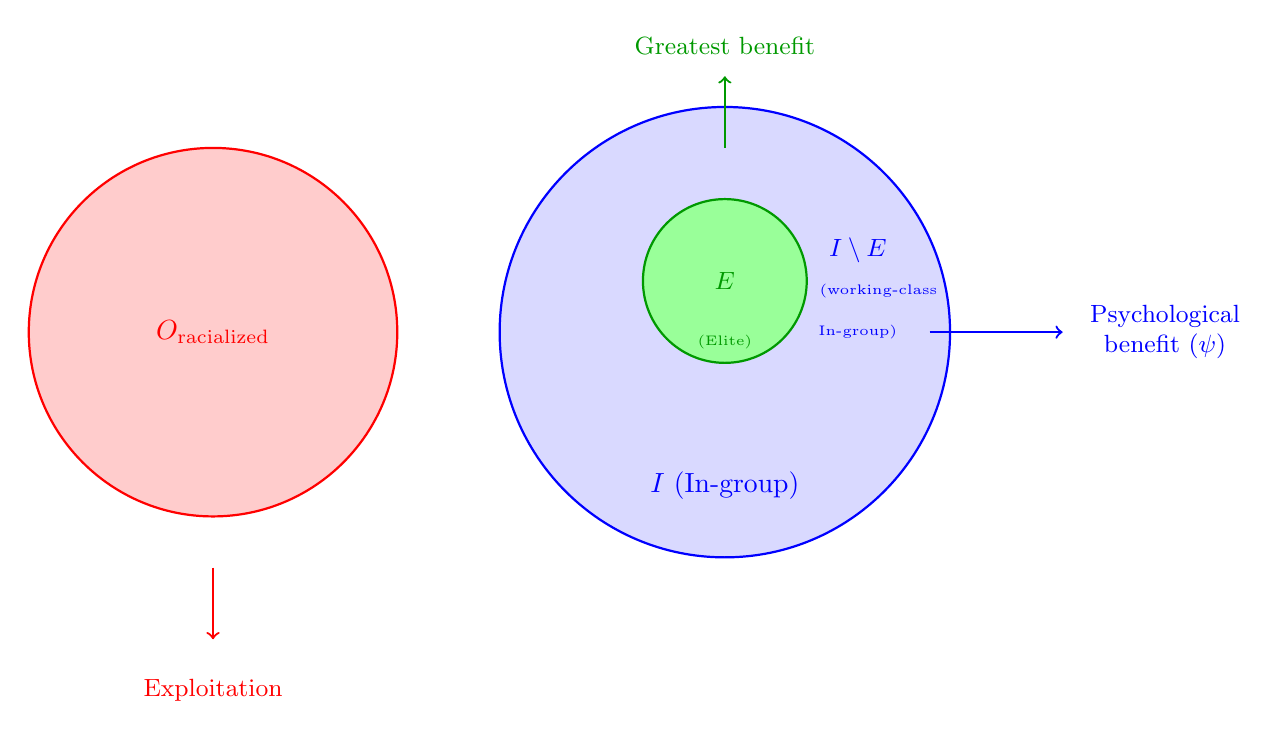
\begin{tikzpicture}[scale=1.3]
    % Draw the Out-group (large circle on left)
    \draw[thick, red, fill=red!20] (-3,0) circle (1.8cm);
    \node[red] at (-3,0) {$O_{\text{racialized}}$};

    % Draw the In-group (large circle on right)
    \draw[thick, blue, fill=blue!15] (2,0) circle (2.2cm);
    \node[blue] at (2,-1.5) {$I$ (In-group)};

    % Draw the Elite (small circle inside In-group)
    \draw[thick, green!60!black, fill=green!40] (2,0.5) circle (0.8cm);
    \node[green!60!black, font=\small] at (2,0.5) {$E$};
    \node[green!60!black, font=\tiny] at (2,-0.1) {(Elite)};

    % Draw the non-Elite In-group region label - moved inside circle, away from boundary
    \node[blue, font=\small] at (3.3,0.8) {$I \setminus E$};
    \node[blue, font=\tiny] at (3.5,0.4) {(working-class};
    \node[blue, font=\tiny] at (3.3,0.0) {In-group)};

    % Arrow annotations showing benefit flow
    \draw[->, thick, green!60!black] (2,1.8) -- (2,2.5);
    % "Greatest benefit" moved above arrow
    \node[green!60!black, font=\small] at (2,2.8) {Greatest benefit};

    % Psychological benefit arrow - shifted right more
    \draw[->, thick, blue] (4.0,0) -- (5.3,0);
    \node[blue, font=\small, align=center] at (6.3,0) {Psychological\\benefit ($\psi$)};

    \draw[->, thick, red] (-3,-2.3) -- (-3,-3);
    \node[red, font=\small] at (-3,-3.5) {Exploitation};
\end{tikzpicture}
\caption{Three-tier model showing Elite ($E$) as a small subset of In-group ($I$), with Out-group ($O_{\text{racialized}}$) exploited to benefit the Elite while $(I \setminus E)$ receives psychological compensation ($\psi$). This is the foundational structure of the system.}
\label{fig:elite_model}
\end{figure}

This three-tier structure is governed by what we term the \textbf{Predatory Min-Max Function}. The system operates according to two imperatives:

\begin{enumerate}
    \item \textbf{Maximize ($Max$):} The extraction of capital, labor, and autonomy from the labor force---primarily from $O_{\text{racialized}}$, but eventually from $I \setminus E$ as well.
    \item \textbf{Minimize ($Min$):} The risk of a unified class revolution against the Elite ($E$), achieved by deploying $\psi$ to keep $I \setminus E$ invested in racial hierarchy rather than class solidarity.
\end{enumerate}

\[
\text{Objective:} \quad \frac{\text{Max}(\text{Extraction})}{\text{Min}(\text{Resistance}_{\text{class}})} \rightarrow \text{System Stability}
\]

Policies ($P$) are the instruments through which this optimization is executed, impacting $O_{\text{racialized}}$, $I \setminus E$, and $E$ in structurally different ways. The remainder of this section formalizes how these policies compound over time; Section~4 then traces the historical algorithm of Elite optimization through six phases.

\textbf{A Note on Scope and Specificity}: This model is specifically designed to analyze racism as a unique system rooted in the 15th century racialization of African peoples for the purposes of enslavement and colonial exploitation. The notation $O_{\text{racialized}}$ reflects this historical specificity. While the mathematical architecture may share structural similarities with other systems of oppression, this paper focuses on racism's particular genealogy and mechanisms. The subscript ``racialized'' anchors the mathematical formalism to the historical narrative established in Section 2, ensuring that the model captures the unique features of racism rather than generic intergroup conflict.

\subsection{Modeling Systemic Racism: From Summation to Compounding}

Traditional approaches might model the cumulative negative impact of policies as simple summation:
\[
\sum (O_{\text{racialized}} \cap P) > \sum ((I \setminus E) \cap P) > \sum (E \cap P)
\]
where the burden of policy falls most heavily on $O_{\text{racialized}}$, partially on the buffer class $I \setminus E$, and least on the Elite $E$ who architect the policies. However, even this three-tiered additive model fails to capture a critical dimension of systemic racism: \textbf{policies compound over time}. Each policy does not merely add harm; it fundamentally alters the vulnerability of the targeted groups to subsequent policies.

To capture this compounding effect, we introduce a temporal model where the state of the Out-group at time $t+1$ depends on its state at time $t$ and the policy enacted:
\[
O_t^{\text{capacity}} = O_{t-1}^{\text{capacity}} \cdot (1 - \alpha P_t)
\]
where $O_t^{\text{capacity}}$ represents the accumulated capital, power, and resources of the Out-group at time $t$, $P_t$ is the policy enacted at time $t$, and $\alpha$ is a coefficient representing the extractive intensity of the policy.

This formulation reveals why historical sequencing matters. Consider two policies, $P_1$ (15th century enslavement) and $P_2$ (20th century redlining):
\[
O_2^{\text{capacity}} = O_0^{\text{capacity}} \cdot (1 - \alpha P_1) \cdot (1 - \beta P_2)
\]
The impact of $P_2$ is applied to an Out-group \textit{already diminished} by $P_1$. If we applied the same policy $P_2$ to a group without the history of $P_1$, the absolute harm would be less severe. This multiplicative effect explains the \textbf{entrenchment} of systemic racism: early oppression doesn't just add disadvantage; it changes the entire equation for all subsequent policies.

Crucially, while $O_{\text{racialized}}$ bears the primary compounding burden, the buffer class $I \setminus E$ is not immune. As the Predatory Min-Max Function exhausts extraction from $O_{\text{racialized}}$, the same compounding logic eventually turns inward: the tools developed to diminish $O_{\text{racialized}}$ are redeployed against $I \setminus E$, whose own capacity then begins to compound downward (see Section~4.7).

\textbf{The Vector Equation of Racism}

Traditional sociological models frequently err by calculating prejudice as a \textit{scalar} quantity---a metric possessing magnitude (emotional weight or individual bias) but lacking a definitive direction. Under the strict parameters of the mathematics of oppression, systemic racism cannot be a scalar; it must be defined as a \textbf{vector}.

A vector possesses both magnitude and a specific, irreversible direction. In systems of domination, this vector flows strictly unidirectionally: from the Elite ($E$) and their enforcement apparatus down through the Buffer Class ($I \setminus E$) and onto the Out-group ($O_{\text{racialized}}$). The prejudice of a marginalized group may carry emotional magnitude, but without the backing of institutional force, state violence, and capital management, it lacks the directional velocity required to enact systemic harm. Therefore:

\[
\vec{R}_{\text{systemic}} = \left\| F_{\text{institutional}} \right\| \cdot \hat{d}_{\text{hierarchy}} \quad \neq \quad \left| \text{prejudice}_{\text{individual}} \right|
\]

Attempting to equate the localized anger of the Out-group with the institutional vector of the Elite is a mathematical fallacy---a category error that confuses a scalar with a vector. True oppression is a top-down, structurally guaranteed compounding force, not a simple summation of interpersonal grievances.

\begin{figure}[htbp]
\centering
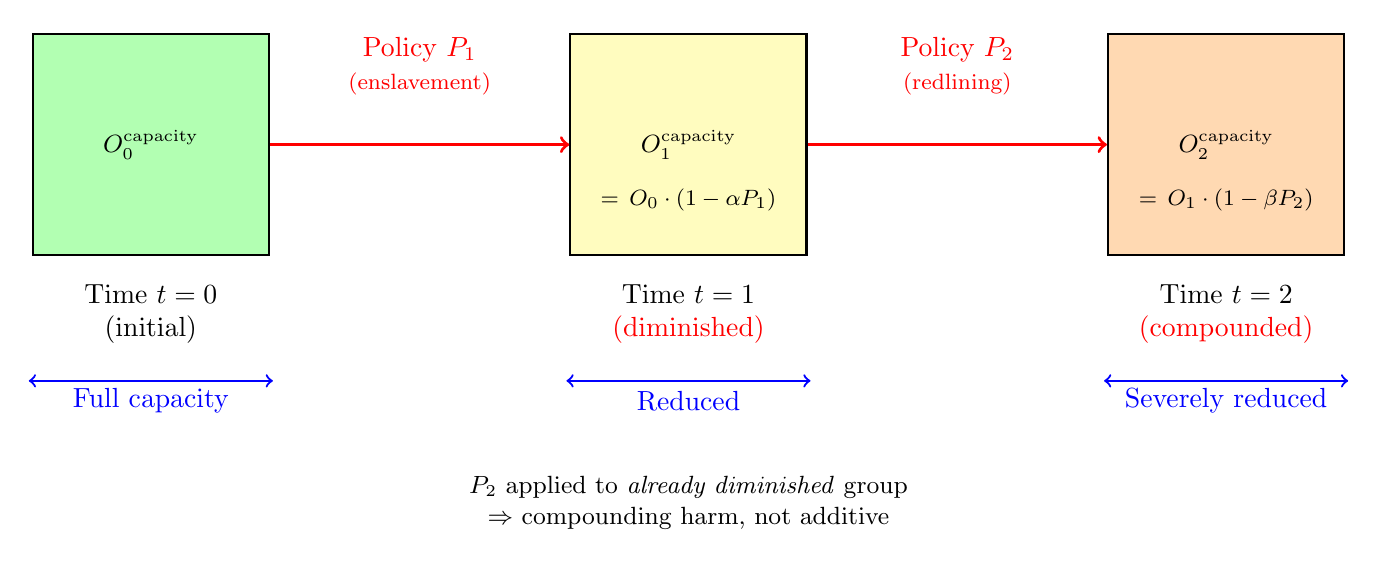
\begin{tikzpicture}[every node/.style={font=\small}]
    % Capacity boxes
    \node[draw, thick, fill=green!30, minimum width=3cm, minimum height=2.8cm] (o0) at (0,0) {$O_0^{\text{capacity}}$};
    \node[draw, thick, fill=yellow!25, minimum width=3cm, minimum height=2.8cm, right=3.8cm of o0] (o1) {$O_1^{\text{capacity}}$};
    \node[draw, thick, fill=orange!30, minimum width=3cm, minimum height=2.8cm, right=3.8cm of o1] (o2) {$O_2^{\text{capacity}}$};

    % Capacity equations
    \node[font=\footnotesize] at ($(o1)+(0,-0.7)$) {$=\, O_0 \cdot (1-\alpha P_1)$};
    \node[font=\footnotesize] at ($(o2)+(0,-0.7)$) {$=\, O_1 \cdot (1-\beta P_2)$};

    % Policy arrows
    \draw[->, very thick, red] (o0.east) -- (o1.west);
    \draw[->, very thick, red] (o1.east) -- (o2.west);
    \node[red, font=\normalsize, align=center] at ($(o0)!0.5!(o1)+(0,1.0)$) {Policy $P_1$\\\footnotesize(enslavement)};
    \node[red, font=\normalsize, align=center] at ($(o1)!0.5!(o2)+(0,1.0)$) {Policy $P_2$\\\footnotesize(redlining)};

    % Time labels
    \node[font=\normalsize] at ($(o0)+(0,-1.9)$) {Time $t=0$};
    \node[font=\normalsize] at ($(o0)+(0,-2.35)$) {(initial)};

    \node[font=\normalsize] at ($(o1)+(0,-1.9)$) {Time $t=1$};
    \node[font=\normalsize, red] at ($(o1)+(0,-2.35)$) {(diminished)};

    \node[font=\normalsize] at ($(o2)+(0,-1.9)$) {Time $t=2$};
    \node[font=\normalsize, red] at ($(o2)+(0,-2.35)$) {(compounded)};

    % Visual representation of shrinking
    \draw[<->, thick, blue] ($(o0)+(-1.55,-3)$) -- ($(o0)+(1.55,-3)$);
    \node[blue, font=\normalsize] at ($(o0)+(0,-3.25)$) {Full capacity};

    \draw[<->, thick, blue] ($(o1)+(-1.55,-3)$) -- ($(o1)+(1.55,-3)$);
    \node[blue, font=\normalsize] at ($(o1)+(0,-3.25)$) {Reduced};

    \draw[<->, thick, blue] ($(o2)+(-1.55,-3)$) -- ($(o2)+(1.55,-3)$);
    \node[blue, font=\normalsize] at ($(o2)+(0,-3.25)$) {Severely reduced};

    % Annotation
    \node[align=center, font=\small] at ($(o1)+(0,-4.55)$) {$P_2$ applied to \textit{already diminished} group\\$\Rightarrow$ compounding harm, not additive};
\end{tikzpicture}
\caption{Temporal compounding model: Each policy reduces Out-group capacity, making subsequent policies more harmful. Policy $P_2$ (redlining) causes greater harm when applied to a group already diminished by $P_1$ (enslavement). As the system exhausts extraction from $O_{\text{racialized}}$, this same compounding mechanism is eventually turned against $I \setminus E$ (Section~4.7).}
\label{fig:compounding}
\end{figure}

\begin{figure}[htbp]
\centering
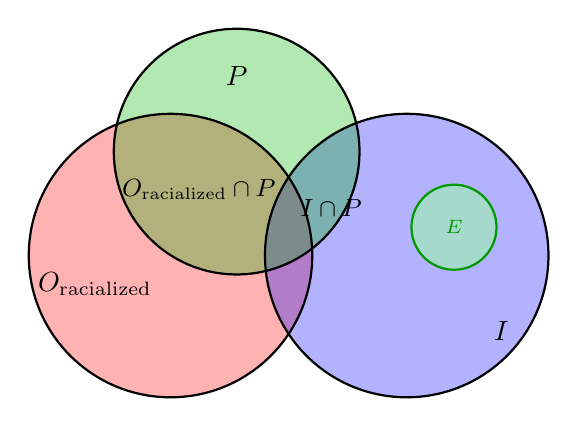
\begin{tikzpicture}[scale=1.2]
    % Define the circles
    \def\circleA{(0,0) circle (1.5cm)}
    \def\circleB{(2.5,0) circle (1.5cm)}
    \def\circleC{(0.7,1.1) circle (1.3cm)}

    % Fill the intersections with different shades
    \begin{scope}[fill opacity=0.3]
        \fill[red] \circleA;
        \fill[blue] \circleB;
        \fill[green!70!black] \circleC;
    \end{scope}

    % Draw the circles
    \draw[thick] \circleA;
    \draw[thick] \circleB;
    \draw[thick] \circleC;

    % Draw Elite as small circle nested inside I
    \draw[thick, green!60!black, fill=green!40, fill opacity=0.5] (3.0,0.3) circle (0.45cm);
    \node[green!60!black, font=\scriptsize] at (3.0,0.3) {$E$};

    % Add labels
    \node at (-0.8,-0.3) {$O_{\text{racialized}}$};
    \node at (3.5,-0.8) {$I$};
    \node at (0.7,1.9) {$P$};

    % Add description of intersections
    \node[align=center, font=\small] at (0.3,0.7) {$O_{\text{racialized}} \cap P$};
    \node[align=center, font=\small] at (1.7,0.5) {$I \cap P$};
\end{tikzpicture}
\caption{Venn diagram illustrating the relationships between the Out-group ($O_{\text{racialized}}$), Policies ($P$), and In-group ($I$), with the Elite ($E \subset I$) shown as a small subset within the In-group. Policies intersect differently with each group, primarily extracting from $O_{\text{racialized}}$ to benefit $E$.}
\label{fig:venn_model}
\end{figure}

\subsection{Historical Policies as Case Studies}

Historical policies, such as the Portuguese slave trade and subsequent colonial practices, serve as real-world examples of our model. These policies created and perpetuated disparities between racial groups, institutionalizing racism at a systemic level.

\subsection{The Three-Tier Dynamics in Detail}

The three-tier model introduced at the opening of this section---with the foundational inequality $\text{Benefit}(E) \gg \text{Benefit}(I \setminus E) > \text{Benefit}(O_{\text{racialized}})$ and the Predatory Min-Max Function governing it---has several important implications worth elaborating.

The psychological wage $\psi$ is not merely a side effect of the system; it is a \textit{designed feature}. The Elite ($E$) invest in $\psi$ precisely because it is cheaper than material concession: granting $I \setminus E$ racial status, legal privileges over $O_{\text{racialized}}$, and the right to police the racial boundary costs the Elite far less than sharing material wealth. This makes $\psi$ the key variable in the Predatory Min-Max Function's minimization of class resistance (see Figure~\ref{fig:elite_model}).

The system thus produces a paradox: $I \setminus E$ defends a hierarchy that materially harms them, because the psychological wage creates the \textit{perception} of shared interest with $E$ and the \textit{perception} of threat from $O_{\text{racialized}}$. Both perceptions serve $E$'s extraction objectives.

\section{The Calculus of Control -- The Optimization of Elite Impunity}

Having established the three-tier model in Section~3---with $\text{Benefit}(E) \gg \text{Benefit}(I \setminus E) > \text{Benefit}(O_{\text{racialized}})$, the psychological wage $\psi$ sustaining the buffer class, and the Predatory Min-Max Function governing the system's optimization---we now trace the \textit{algorithm} of this optimization through history. The historical timeline reveals that the In-group was artificially constructed to solve a specific security flaw. Once the extraction of the Out-group ($O_{\text{racialized}}$) is exhausted, the system inevitably \textbf{cannibalizes} the buffer class it created. We can map this algorithm through six distinct phases of optimization (see Figure~\ref{fig:extraction_zone}).

\subsection{The Source Code: Portuguese Origins (1450s)}
As detailed in Section 2, the ideological ``source code'' for racism was written in 1450s Portugal. The key insight, rendered in algorithmic terms: the European Elite could not extract unlimited labor from a population that shared their moral community ($I_{\text{Christendom}}$). Zurara's racialization of African peoples (Section 2.2) solved this by creating a new category---a fungible Out-group ($O$) defined outside the moral community entirely.

\begin{itemize}
    \item \textbf{The Function:} Group all disparate African peoples into a single category defined by \textit{lack} (lack of salvation, lack of civilization), bypassing the moral and social constraints of European labor relations.
    \item \textbf{The License:} When the first enslaved Africans arrived in Virginia in 1619---stolen from the Portuguese slave ship \textit{San Juan Bautista}---the English colonists did not need to write the logic of chattel slavery from scratch. They simply licensed the Portuguese algorithm.
\end{itemize}

\subsection{The Application: Bacon's Rebellion and the Partition of the Poor (1676)}
In the American colonies, however, the Elite initially failed to implement this code strictly. The "proto-working class" was a mix of European indentured servants ($L_{white}$) and enslaved Africans ($L_{black}$). Because they shared the same oppressive conditions, the Portuguese distinction didn't stop them from seeing each other as allies.

This led to the system crash of \textbf{Bacon's Rebellion (1676)}. The united Labor Class ($L_{white} \cup L_{black}$) burned Jamestown to the ground, proving that:

\[
\text{If} \quad (L_{white} + L_{black}) > E \quad \rightarrow \quad \text{Revolution}
\]

\subsection{The Patch: The Invention of "Whiteness" (1705)}
To prevent a recurrence, the Virginian Elite \textbf{weaponized the Portuguese code}. They enacted the \textbf{Virginia Slave Codes of 1705}, which explicitly created a legal wall between the two groups \cite{allen, kendi}.

\begin{enumerate}
    \item \textbf{The Partition:} They assigned $L_{white}$ to a new category: "White."
    \item \textbf{The Bribe:} They gave the poor whites the psychological wage $\psi$ (Section~3)---the right to police the Black population, the right to bear arms, and immunity from chattel slavery.
\end{enumerate}

This was the masterstroke of the American algorithm: It used "Race" to destroy "Class." It recruited the poor white population to act as the \textbf{Buffer Class}, protecting the Elite from the very people they should have been allied with.

\[
\text{Buffer Created:} \quad I_{poor} \rightarrow \text{Defender of } E
\]

\subsection{The System Kernel: The 13th Amendment Loophole (1865)}
Following the Civil War, the system required a new legal kernel. The \textbf{13th Amendment} converted slavery from a static identity to a conditional state via the exception clause: \textit{``except as a punishment for crime''} \cite{alexander, blackmon, thirteenth}.

\[
\text{If} \quad \text{Status}(x) = \text{Criminal}(C) \quad \rightarrow \quad \text{Status}(x) \in S \text{ (Slave)}
\]

This ensured that slavery remained a constitutionally protected state, accessible to the Elite as long as they could map the target population to the variable of Criminality ($C$).

\subsubsection*{Case Study: The Governor's Mansion and the Normalization of the 13th Amendment Loophole}

The transition from chattel slavery to the carceral extraction of the 13th Amendment loophole was not a hidden conspiracy; it was---and remains---a celebrated feature of the political interface.

To understand how thoroughly this extraction has been normalized by the political class ($P_{\text{puppet}} \subset E$), one need look no further than the Arkansas Governor's Mansion. In her 1996 memoir, former First Lady Hillary Clinton detailed the ``longstanding tradition'' of using prison inmates to staff the residence. She explicitly noted that this practice ``kept down costs'' and that the mansion was largely maintained by a few ``African-American men in their thirties'' who cooked and cleaned for the family \cite{clinton_village}.

This was not a wage-labor arrangement; it was the 13th Amendment exception clause in perfect, unvarnished operation. The laborers worked under strict compulsion. As Clinton noted, any inmate who broke a rule was immediately ``sent back to prison.'' The threat of the carceral cage served as the absolute guarantor of compliance and free labor.

Crucially, this practice is not isolated to one political family. As investigative journalists have repeatedly documented, the use of uncompensated or violently under-compensated carceral labor in governors' mansions is a bipartisan tradition across the United States \cite{currentaffairs_slaves}. The Clintons are notable only because they documented it so casually.

When the political elite can publicly write about utilizing uncompensated Black men to serve their households to ``keep down costs''---and face zero societal backlash---it proves that the ideological justification of the extraction algorithm is complete. The system did not abolish the plantation; it simply state-sponsored it.

\subsubsection*{The Algorithm Resists: The 2026 Colorado Ruling}

The bipartisan normalization of carceral labor is so deeply embedded in the extraction engine that even direct democratic intervention struggles to dismantle it.

Consider the system's response when the Buffer Class ($I \setminus E$) and the Out-group ($O$) successfully unite to patch the code. In 2018, Colorado voters passed a constitutional amendment explicitly eliminating the 13th Amendment exception clause, legally abolishing slavery and involuntary servitude as criminal punishment within the state. Theoretically, the extraction kernel should have crashed.

Instead, the system simply ignored the electorate. The Colorado Department of Corrections---operating as the state's enforcement arm ($F_{\text{enforce}}$)---continued to compel incarcerated individuals to work \cite{colorado_forced_labor}. When the legal justification was removed, they relied entirely on raw physical coercion, threatening those who refused to labor with extreme punitive measures such as solitary confinement.

It took additional years of litigation, culminating in a February 2026 court ruling, to finally declare the forced labor unconstitutional. This timeline provides a vital mathematical proof for our framework: \textit{changing the legal interface is not enough}. The political class ($P_{\text{puppet}}$) and its enforcement arms are so dependent on the economic subsidy of the Out-group's forced labor that they will actively violate their own constitutional amendments to keep the extraction engine running.

\subsection{The Optimization: Redlining as the Containment Field (1934)}
To safely harvest the Out-group ($O$) using this criminalization kernel without accidentally capturing the white buffer class ($I_{poor}$), the Elite required a \textbf{Geospatial Targeting Grid}.

\textbf{Redlining} (1934) concentrated Black poverty into urban zones while subsidizing White flight to the suburbs \cite{rothstein, coatesreparations}. This was not benevolence toward whites; it was \textbf{blast radius management}. It ensured that when the state deployed predatory extraction (policing/fines), the "collateral damage" to the white working class would be minimized, preventing a recurrence of the shared grievances that triggered Bacon's Rebellion.

\subsubsection*{The Audible Firewall of 1959}

\textbf{The 1959 Archive: Defending the Psychological Wage}

To understand the sheer structural power of the psychological wage ($\psi$), one must examine the historical friction of the Civil Rights era---not from the perspective of the policymakers, but from the mouths of the Buffer Class ($I_{\text{buffer}} = I \setminus E$) themselves.

In a January 21, 1959 broadcast titled ``Students and Parents Speak Out about Integration,'' white working- and middle-class citizens articulated their visceral resistance to the desegregation of public schools. While conventionally analyzed as a tragic display of interpersonal prejudice (the downstream exhaust of the system), within the Predatory Min-Max Function, this audio serves as a pristine diagnostic of the algorithm functioning flawlessly.

What the 1959 broadcast captures is the absolute terror of a class defending its only asset. Because the Elite ($E$) had systematically extracted the material wealth of the white working class, the artificial social elevation \textit{over} the Out-group ($O_{\text{racialized}}$) was the only compensation $I_{\text{buffer}}$ possessed. Integration threatened to mathematically equalize the spatial and educational environments of $I_{\text{buffer}}$ and $O_{\text{racialized}}$, effectively dropping the value of $\psi$ to zero.

Crucially, note who is \textit{absent} from these historical integration protests: the Elite. The hyper-concentrated capital class did not need to stand in front of public schools screaming at Black children. They had already secluded their own children in heavily capitalized, elite private academies. Instead, they successfully outsourced the kinetic enforcement of the racial boundary to the Buffer Class.

The 1959 broadcast is the literal sound of the Johnson Theorem in action. It is the sound of the ``lowest white man'' fiercely defending the exact hierarchy that keeps his own pockets empty, fighting a war against the Out-group to protect an ideological shield manufactured by the Elite. It proves that the system's firewall is self-sustaining: once the psychological wage is distributed, the Buffer Class will physically riot to maintain their own subjugation.

\subsection{The Interface Shift: The War on Drugs (1968)}
When \textit{Brown v. Board} (1954) blocked the use of explicit racial laws, the Nixon Administration executed the \textbf{Variable Swap}. As John Ehrlichman admitted, they used the \textbf{War on Drugs} to associate ``blacks with heroin'' and ``hippies with marijuana'' \cite{baum, vera, alexander}.

This expanded the Out-group to include political dissidents from the In-group, while Lee Atwater's \textbf{``Dog Whistle''} strategy (1981) provided the abstract language (``State's Rights,'' ``Law and Order'') to mask the operation from the white public \cite{lopez, phillips}.

\subsubsection*{The Educational Rug Pull and the $P_{\text{debt}}$ Proxy}

\textbf{The Educational Interface Swap: From Segregation to $P_{\text{debt}}$}

When the legal mechanisms of educational segregation were finally dismantled, the Elite ($E$) required a new filter to prevent the Out-group ($O_{\text{racialized}}$) from achieving economic parity. The system executed a seamless \textbf{Interface Swap}: replacing explicit racial exclusion with an exorbitant Economic Filter.

The political class ($P_{\text{puppet}}$) allowed the cost of higher education to hyper-inflate. This was not an accident of the free market; it was a calculated exploitation of the compounding equation established in Section~3.1. Because the In-group possessed centuries of accumulated capital ($I^{t}_{\text{capacity}}$)---built through redlining, generational inheritance, and subsidized housing---they could absorb the hyper-inflated costs of college. The Out-group, having been systematically stripped of generational wealth, could not.

However, the system's true malice lies in its \textit{false promise of access}. The Out-group was told they could finally enter the halls of higher education, but only if they subjected themselves to the $P_{\text{debt}}$ variable.

Much like the 1825 Independence Debt forced upon Haiti (where the emancipated Out-group was forced to literally purchase their own stolen autonomy at gunpoint), the modern student loan system is a form of \textbf{individual sovereign ransom}. A member of $O_{\text{racialized}}$ attempting to achieve class mobility does not start at zero; they are forced to start deep in the negative, pledging decades of their future labor to Elite-controlled financial institutions just to access the baseline economy.

But the algorithm contains one final, devastating trap: \textbf{The Depreciating Asset}.

Once the Out-group successfully debt-financed their way into higher education, the Elite simply moved the goalposts. They depreciated the value of the undergraduate degree itself. A credential that once guaranteed entry into the middle class for the Buffer Class was mathematically devalued, \textit{replaced} by new gatekeeping mechanisms: unpaid internships, elite social networks, and master's degree requirements.

The Out-group is thus left holding a hyper-inflated mortgage on a depreciated asset. The debt cannot be discharged in bankruptcy, ensuring that even when the Out-group ``plays by the rules'' and achieves the education, they remain mathematically tethered to the extraction kernel, functionally identical to indentured labor.

\subsection{The Collapse: Cannibalizing the In-Group (Present)}
This brings us to the final, inevitable stage of the algorithm. An extraction system requires \textbf{Infinite Growth}. Once the Out-group ($O$) has been fully harvested---stripped of wealth, voting rights, and labor \cite{coates}---the Elite ($E$) must find new sources of extraction to maintain their accumulation.

The system has now turned inward. The tools developed to oppress the Out-group are being deployed against the In-group:
\begin{itemize}
    \item \textbf{The Opioid Crisis:} The criminalization of white addiction mirrors the crack epidemic.
    \item \textbf{Militarized Policing:} SWAT tactics invented for the "Ghetto" are now used in rural towns.
    \item \textbf{Surveillance:} The loss of privacy tested on the poor is now applied to the middle class.
\end{itemize}

\subsubsection*{The Algorithmic Commodification of Suffering}

The extraction algorithm, which historically manifested in physical labor and territorial conquest, has evolved into a highly abstracted data model. In the modern digital and military-industrial era, the Out-group's physical suffering is directly converted into \textbf{predictive capital}.

Consider the geospatial data generated by a marginalized population undergoing kinetic military bombardment or intensive state policing. The panic, the irregular movement patterns, and the desperate communication attempts produce massive, proprietary datasets. Technological contractors harvest this behavioral data to train advanced AI algorithms---such as emergency response or crowd-control software---which are then sold at a premium to global governments and healthcare systems.

In this updated calculus, the Out-group is no longer extracted solely for their labor; their very \textit{trauma} is mathematically commodified:

\[
\text{Extraction}_{t_{\text{modern}}} = \underbrace{\text{Labor}(O)}_{\text{traditional}} + \underbrace{\text{Data}(\text{Suffering}(O))}_{\text{digital frontier}}
\]

This proves that the Elite's extraction algorithm is continually optimizing for new frontiers of profit. The system does not grow a conscience; it grows new markets.

\subsubsection*{Conclusion}
The ``White Working Class'' was never a partner to the Elite; they were merely the \textbf{Reserve Food Supply}. By accepting the bribe of ``Whiteness'' in 1705, they agreed to police the prison that is now expanding to hold \textit{them}.

The definition of the Out-group has returned to its 1676 state:

\[
O_{final} = \text{Everyone} \setminus E
\]

\begin{figure}[h]
    \centering
    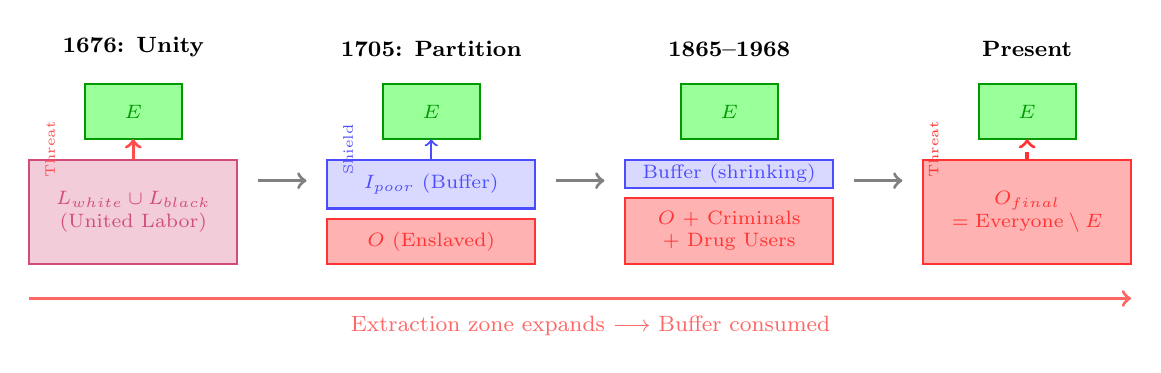
\begin{tikzpicture}[scale=0.88, every node/.style={font=\small}]

    % --- Phase 1: 1676 (United labor) ---
    \begin{scope}[shift={(0,0)}]
        \node[font=\footnotesize\bfseries, anchor=south] at (1.5,2.85) {1676: Unity};
        % Elite box
        \draw[thick, green!60!black, fill=green!40] (0.8,1.8) rectangle (2.2,2.6);
        \node[green!60!black, font=\scriptsize] at (1.5,2.2) {$E$};
        % United labor
        \draw[thick, purple!70, fill=purple!20] (0,0) rectangle (3,1.5);
        \node[purple!70, font=\scriptsize, align=center] at (1.5,0.75) {$L_{white} \cup L_{black}$\\(United Labor)};
        % Threat arrow
        \draw[->, very thick, red!70] (1.5,1.5) -- (1.5,1.8);
        \node[red!70, font=\tiny, rotate=90] at (0.3,1.65) {Threat};
    \end{scope}

    % Arrow
    \draw[->, very thick, gray] (3.3,1.2) -- (4.0,1.2);

    % --- Phase 2: 1705 (Partition) ---
    \begin{scope}[shift={(4.3,0)}]
        \node[font=\footnotesize\bfseries, anchor=south] at (1.5,2.85) {1705: Partition};
        % Elite box
        \draw[thick, green!60!black, fill=green!40] (0.8,1.8) rectangle (2.2,2.6);
        \node[green!60!black, font=\scriptsize] at (1.5,2.2) {$E$};
        % Buffer class (white)
        \draw[thick, blue!70, fill=blue!15] (0,0.8) rectangle (3,1.5);
        \node[blue!70, font=\scriptsize] at (1.5,1.15) {$I_{poor}$ (Buffer)};
        % Extraction zone (black)
        \draw[thick, red!80, fill=red!30] (0,0) rectangle (3,0.65);
        \node[red!80, font=\scriptsize] at (1.5,0.32) {$O$ (Enslaved)};
        % Shield arrow
        \draw[->, thick, blue!70] (1.5,1.5) -- (1.5,1.8);
        \node[blue!70, font=\tiny, rotate=90] at (0.3,1.65) {Shield};
    \end{scope}

    % Arrow
    \draw[->, very thick, gray] (7.6,1.2) -- (8.3,1.2);

    % --- Phase 3: 1865--1968 (Expansion) ---
    \begin{scope}[shift={(8.6,0)}]
        \node[font=\footnotesize\bfseries, anchor=south] at (1.5,2.85) {1865--1968};
        % Elite box
        \draw[thick, green!60!black, fill=green!40] (0.8,1.8) rectangle (2.2,2.6);
        \node[green!60!black, font=\scriptsize] at (1.5,2.2) {$E$};
        % Buffer class (shrinking)
        \draw[thick, blue!70, fill=blue!15] (0,1.1) rectangle (3,1.5);
        \node[blue!70, font=\scriptsize] at (1.5,1.3) {Buffer (shrinking)};
        % Expanded extraction zone
        \draw[thick, red!80, fill=red!30] (0,0) rectangle (3,0.95);
        \node[red!80, font=\scriptsize, align=center] at (1.5,0.48) {$O$ + Criminals\\+ Drug Users};
    \end{scope}

    % Arrow
    \draw[->, very thick, gray] (11.9,1.2) -- (12.6,1.2);

    % --- Phase 4: Present (Cannibalization) ---
    \begin{scope}[shift={(12.9,0)}]
        \node[font=\footnotesize\bfseries, anchor=south] at (1.5,2.85) {Present};
        % Elite box
        \draw[thick, green!60!black, fill=green!40] (0.8,1.8) rectangle (2.2,2.6);
        \node[green!60!black, font=\scriptsize] at (1.5,2.2) {$E$};
        % Extraction zone consuming nearly everything
        \draw[thick, red!80, fill=red!30] (0,0) rectangle (3,1.5);
        \node[red!80, font=\scriptsize, align=center] at (1.5,0.75) {$O_{final}$\\$= \text{Everyone} \setminus E$};
        % Cannibalization arrow
        \draw[->, very thick, red!80, dashed] (1.5,1.5) -- (1.5,1.8);
        \node[red!80, font=\tiny, rotate=90] at (0.15,1.65) {Threat};
    \end{scope}

    % Bottom annotation
    \draw[->, very thick, red!60] (0,-0.5) -- (15.9,-0.5);
    \node[red!60, font=\footnotesize, anchor=west] at (4.5,-0.9) {Extraction zone expands $\longrightarrow$ Buffer consumed};

    \end{tikzpicture}
    \caption{\textbf{The Recursive Expansion of the Extraction Zone (1676--Present).} This diagram illustrates the ``Min-Max'' algorithm in motion. Following the threat of unity in 1676, the Elite created a racial partition to separate the labor force. However, as the extraction system requires infinite growth, the ``Out-group'' ($O$) has progressively expanded---first capturing Black bodies via chattel slavery, then criminalized populations via the War on Drugs, and finally cannibalizing the white working class via the modern surveillance and opioid crises. The ``Buffer Class'' ($I$) was never a permanent partner to the Elite, but a temporary reserve of capital.}
    \label{fig:extraction_zone}
\end{figure}

\section{From Diagnosis to Prescription: Policy Implications}

The algorithmic history traced in Section 4 is not merely descriptive---it is \textit{diagnostic}. Each phase of the Elite's optimization (Portuguese racialization $\rightarrow$ Bacon's Rebellion $\rightarrow$ the invention of whiteness $\rightarrow$ the 13th Amendment loophole $\rightarrow$ redlining $\rightarrow$ the War on Drugs $\rightarrow$ cannibalization) reveals a system that adapts its \textit{interface} while preserving its \textit{kernel}: the Predatory Min-Max Function that maximizes extraction while minimizing class resistance.

If the framework is correct, it does not merely describe racism---it \textit{prescribes} specific interventions by revealing where harm is concentrated and how it operates. This section examines what follows from the model.

\subsection{Policy Implications: Individual vs.\ Systemic Interventions}

The mathematical framework developed here does not merely describe racism---it \textit{prescribes} specific interventions by revealing where harm is concentrated and how it operates. This framework forces a fundamental shift from individual-focused solutions to systemic policy reform.

\textbf{The Failure of Individual-Focused Solutions}

Traditional approaches to addressing racism often focus on individual prejudice and bias. In the case of lending disparities, for example, this approach leads to interventions such as:
\begin{itemize}
    \item Sensitivity training for loan officers
    \item Implicit bias workshops
    \item Diversity hiring initiatives
    \item Individual complaint mechanisms
\end{itemize}

While these interventions may address individual instances of discrimination, our mathematical model reveals why they cannot address systemic racism. The model identifies the \textit{intersection} $O_{\text{racialized}} \cap P$ as the site of greatest harm. Individual-focused solutions attempt to modify the behavior of actors \textit{within} the system while leaving the policy $P$ unchanged. Mathematically, this is attempting to reduce harm while keeping the structural inequality intact.

Moreover, our temporal compounding model demonstrates that individual bias is \textit{downstream} of systemic design. The accumulated disadvantage represented by $O_t^{\text{capacity}}$ creates disparities that appear even when individual actors have no conscious bias. A loan officer applying ostensibly neutral criteria to applicants with dramatically different accumulated capital (due to historical policies like redlining, employment discrimination, and wealth extraction) will produce racially disparate outcomes even with zero individual prejudice.

\textbf{Systemic Interventions Mandated by the Framework}

Our framework compels a fundamentally different approach. By identifying $O_{\text{racialized}} \cap P$ as the mathematical site of harm, the framework mandates direct intervention on the \textit{policy} $P$ itself:

\textbf{Case Study: Lending Disparities}

The framework demands an audit of the institutional rules and underwriting criteria that constitute $P$. Specific interventions include:
\begin{enumerate}
    \item \textbf{Audit the policy structure}: Examine whether underwriting criteria (credit score thresholds, debt-to-income ratios, down payment requirements, employment history requirements) structurally disadvantage groups with diminished $O_t^{\text{capacity}}$ due to historical policies.
    
    \item \textbf{Measure the intersection}: Quantify $|O_{\text{racialized}} \cap P_{\text{current}}|$---the number of Out-group members adversely affected by current policy---and compare to $|I \cap P_{\text{current}}|$.
    
    \item \textbf{Redesign policy parameters}: Modify $P$ to reduce the intersection's size. For example, if credit score thresholds disproportionately exclude the Out-group due to historical policies that limited their access to credit, the framework mandates adjusting the threshold or using alternative metrics.
    
    \item \textbf{Validate structural change}: Demonstrate mathematically that the modified policy $P'$ produces:
    \[
    |O_{\text{racialized}} \cap P'| < |O_{\text{racialized}} \cap P|
    \]
    A reduction in the intersection represents structural improvement, regardless of individual attitudes.
\end{enumerate}

\textbf{Predictive Power of the Framework}

The framework makes individual-focused solutions \textit{mathematically predictable failures}. If the policy $P$ structurally targets the Out-group---that is, if $|O_{\text{racialized}} \cap P| \gg |I \cap P|$ by design---then modifying individual behavior within that system cannot eliminate the disparity. The inequality is built into the policy's structure.

This shifts the analytical focus from ``Do individual actors harbor bias?'' to ``Is this policy $P$ inherently unequal in its design?'' If the answer is yes, the policy must change. Period. No amount of training, awareness, or individual reform can substitute for structural policy transformation.

\textbf{Expanding the Framework}

This analytical approach applies to any domain where racial disparities exist:
\begin{itemize}
    \item \textbf{Criminal `injustice'}: Rather than focusing on individual police officer bias, audit the policies (stop-and-frisk, broken windows policing, mandatory minimums) that constitute $P$ and measure their intersection with $O_{\text{racialized}}$.
    \item \textbf{Education}: Rather than diversity initiatives alone, examine funding formulas, attendance boundaries, and admission criteria that constitute $P$ in educational systems.
    \item \textbf{Employment}: Rather than unconscious bias training, audit job requirements, salary structures, and promotion criteria that disproportionately affect $O_{\text{racialized}}$.
\end{itemize}

The framework's utility lies in its capacity to \textit{compel} specific actions. By mathematically identifying the intersection $O_{\text{racialized}} \cap P$ as the site of harm, it makes policy reform non-negotiable for anyone who accepts the model's premises. This transforms the debate from abstract discussions of racism to concrete, measurable policy interventions with quantifiable outcomes.

\section{Revised Definition of Racism}

Based on our analysis, we propose the following definition:

\begin{quote}
\textbf{Racism} (n.): A system of oppression predicated on the categorization of human beings into ``races'' with perceived inherent differences. This system, rooted in historical practices of enslavement and colonialism, exploits social, economic, and political policies to perpetuate and exacerbate inequalities between racially defined groups. While ostensibly benefiting a racial In-group at the expense of an Out-group, the system primarily serves an Elite class ($E \subset I$) that uses racial division to prevent cross-racial solidarity and to maintain a subjugated labor class. The Out-group targeted by this system tends to \textit{expand} over time, progressively encompassing members of the nominal In-group, revealing that racism ultimately serves Elite economic interests rather than the broader In-group. It is justified through spurious scientific, cultural, and moral claims that obscure this fundamental dynamic.
\end{quote}

\section{Discussion}

This expanded definition and the accompanying mathematical model underscore the systemic, structural nature of racism. This perspective challenges the reduction of racism to individual prejudice, highlighting the historical and ongoing policies that sustain racial inequalities.

However, our set-theoretic analysis reveals something more profound: the conventional framing of racism as a system that benefits whites at the expense of Blacks, while capturing an important dimension of the phenomenon, obscures the deeper structure of exploitation. The introduction of the Elite class ($E$) into our model demonstrates that:

\begin{enumerate}
    \item The true beneficiaries of systemic racism constitute a small subset of the nominal In-group
    \item The broader In-group receives primarily psychological rather than material benefits
    \item The Out-group has consistently \textit{expanded} throughout American history
    \item This expansion increasingly encompasses members of the former In-group
\end{enumerate}

The algorithmic trajectory traced in Section 4---from Portuguese racialization (1450s) through Bacon's Rebellion (1676), the invention of whiteness (1705), the 13th Amendment loophole (1865), redlining (1934), the War on Drugs (1968), and present-day cannibalization of the In-group---demonstrates not a static system of racial oppression but a dynamic one that periodically resets and expands its target population. Each ``reset'' occurs when the previous arrangement becomes untenable: Bacon's Rebellion prompted the invention of rigid racial categories; \textit{Brown v.\ Board} prompted the Variable Swap of the War on Drugs; and the current period of extreme inequality is prompting the cannibalization phase, in which tools built to oppress $O_{\text{racialized}}$ are deployed against $I \setminus E$.

The constitutional mechanism identified in Section 2.6 is particularly insidious: by continuously expanding what constitutes ``crime'' and stripping rights from those convicted via the 13th Amendment's exception clause (Section 4.4), the system can grow the Out-group without ever explicitly naming racial or class categories. The criminalization kernel---$\text{If } \text{Status}(x) = \text{Criminal}(C) \rightarrow \text{Status}(x) \in S$---creates a permanent underclass that crosses racial lines while still disproportionately affecting $O_{\text{racialized}}$.

This pattern suggests we are witnessing another such reset. As economic inequality approaches levels not seen since before the Great Depression, and as automation and globalization eliminate traditional pathways to middle-class stability, the system requires an expanded subjugated class. The Predatory Min-Max Function demands new sources of extraction, and the buffer class created in 1705 is no longer exempt. As formalized in Section 4.7:
\[
O_{\text{final}} = \text{Everyone} \setminus E
\]
This points toward a future where the Out-group continues to grow unless structural intervention disrupts the algorithm.

The incorporation of set theory into our analysis provides more than a quantitative tool; it reveals the \textit{logic} of systemic oppression. Racism is not an aberration or a failure of the American system---it is a \textit{feature} designed to prevent the kind of cross-racial class solidarity that briefly emerged in Bacon's Rebellion and threatened to emerge again during the Civil Rights era \cite{robinson, allen, bonillasilva}.

\section{Conclusion}

Redefining racism to encompass its systemic dimensions and historical roots offers a more comprehensive understanding of the issue, illuminating the pathways through which racial inequalities are perpetuated. More importantly, the Predatory Min-Max Function formalized in Section 4 reveals that the system's governing logic---maximizing extraction while minimizing class resistance---inevitably drives the expansion of the Out-group toward $O_{\text{final}} = \text{Everyone} \setminus E$.

This framework has significant implications for anti-racist strategy. If racism operates as an Elite optimization algorithm that uses racial division to prevent class solidarity, then combating racism requires not only addressing racial disparities but also building coalitions across racial lines that recognize shared economic interests. The ``wages of whiteness''---the psychological bribe offered to $I \setminus E$ in exchange for policing the buffer (Section 4.3)---must be exposed as a poor bargain that leaves them increasingly vulnerable to the same systems of extraction.

The algorithmic trajectory we have documented is not inevitable. The expansion of the Out-group can be halted and reversed through:
\begin{itemize}
    \item Policies that reduce economic inequality and expand the middle class across racial lines
    \item Criminal `injustice' reform that shrinks rather than expands the carceral state
    \item Labor protections that benefit workers regardless of race
    \item Educational efforts that expose the Elite's use of racial division
    \item Coalition-building that emphasizes shared interests over racial grievance
\end{itemize}

The history of American racism, properly understood through the algorithmic lens developed here, is not merely a story of white supremacy but of Elite supremacy maintained through racial division. As long as ordinary members of $I \setminus E$ can be convinced that their interests align with $E$ rather than with $O_{\text{racialized}}$, the Predatory Min-Max Function will continue to optimize---and the extraction zone will continue to expand.

The battle against systemic racism is thus inseparable from the battle against systemic economic exploitation. By embracing this expanded understanding, scholars, policymakers, and the public can engage more effectively in the fight for justice---recognizing that the liberation of the Out-group and the liberation of the broader In-group from Elite manipulation are ultimately the same struggle.

Through a committed and unified approach that transcends racial division, we can aspire to create a society where no group is systematically oppressed to benefit another---including the small Elite that has, for centuries, profited from keeping the rest of us divided.

\begin{thebibliography}{99}

% --- Primary Sources on the Invention of Race and Portuguese Origins ---

\bibitem{kendi}
Kendi, I.X. \textit{Stamped from the Beginning: The Definitive History of Racist Ideas in America}. New York: Nation Books, 2016.

\bibitem{zurara}
Zurara, G.E. de. \textit{Chr\'{o}nica do Descobrimento e Conquista da Guin\'{e}} [Chronicle of the Discovery and Conquest of Guinea]. Written 1453; first published Paris, 1841.

\bibitem{biewen}
Biewen, J. \textit{The Lie That Invented Racism}. TED Talk. Available at: \url{https://ted.com/talks/john_biewen_the_lie_that_invented_racism}

% --- Papal Bulls and Church Authorization ---

\bibitem{dumdiversas}
Pope Nicholas V. \textit{Dum Diversas}. Papal Bull, 18 June 1452.

\bibitem{romanuspontifex}
Pope Nicholas V. \textit{Romanus Pontifex}. Papal Bull, 8 January 1455.

% --- Bacon's Rebellion, the Invention of Whiteness, and Class Solidarity ---

\bibitem{allen}
Allen, T.W. \textit{The Invention of the White Race}. 2 vols. London: Verso, 1994--1997.

\bibitem{roediger}
Roediger, D.R. \textit{The Wages of Whiteness: Race and the Making of the American Working Class}. London: Verso, 1991.

\bibitem{dubois}
Du~Bois, W.E.B. \textit{Black Reconstruction in America, 1860--1880}. New York: Harcourt, Brace and Company, 1935.

% --- Scientific Racism, Eugenics, and Racial Taxonomy ---

\bibitem{gould}
Gould, S.J. \textit{The Mismeasure of Man}. Rev.\ ed. New York: W.W.\ Norton, 1996.

\bibitem{washington}
Washington, H.A. \textit{Medical Apartheid: The Dark History of Medical Experimentation on Black Americans from Colonial Times to the Present}. New York: Doubleday, 2006.

% --- Slavery, the 13th Amendment, and Convict Leasing ---

\bibitem{blackmon}
Blackmon, D.A. \textit{Slavery by Another Name: The Re-Enslavement of Black Americans from the Civil War to World War II}. New York: Doubleday, 2008.

\bibitem{baptist}
Baptist, E.E. \textit{The Half Has Never Been Told: Slavery and the Making of American Capitalism}. New York: Basic Books, 2014.

\bibitem{alexander}
Alexander, M. \textit{The New Jim Crow: Mass Incarceration in the Age of Colorblindness}. New York: The New Press, 2010.

\bibitem{thirteenth}
DuVernay, A. (Director). \textit{13th} [Documentary]. Netflix, 2016.

% --- 13th Amendment Case Studies: Governor's Mansion and Colorado ---

\bibitem{clinton_village}
Clinton, H.R. \textit{It Takes a Village: And Other Lessons Children Teach Us}. New York: Simon \& Schuster, 1996. Ch.~4: ``The Bell Curve Is a Curve Ball.''

\bibitem{currentaffairs_slaves}
Robinson, N.J. ``The Clintons Had Slaves.'' \textit{Current Affairs}, June 2017.

\bibitem{colorado_forced_labor}
\textit{Forced Prison Labor Ruled Unconstitutional in Colorado Following 2018 Anti-Slavery Amendment}. Court ruling, February 2026.

% --- Redlining, Housing Discrimination, and Geospatial Targeting ---

\bibitem{rothstein}
Rothstein, R. \textit{The Color of Law: A Forgotten History of How Our Government Segregated America}. New York: Liveright, 2017.

\bibitem{coatesreparations}
Coates, T.-N. ``The Case for Reparations.'' \textit{The Atlantic}, June 2014.

% --- War on Drugs, Southern Strategy, and Dog Whistle Politics ---

\bibitem{baum}
Baum, D. ``Legalize It All.'' \textit{Harper's Magazine}, April 2016.

\bibitem{vera}
Vera Institute of Justice. \textit{Drug War Confessional}. (Web feature quoting Ehrlichman; accessed 2026). Available at: \url{https://www.vera.org/reimagining-prison-webumentary/the-past-is-never-dead/drug-war-confessional}

\bibitem{lopez}
Haney L\'{o}pez, I. \textit{Dog Whistle Politics: How Coded Racial Appeals Have Reinvented Racism and Wrecked the Middle Class}. Oxford: Oxford University Press, 2014.

\bibitem{phillips}
Phillips, K.P. \textit{The Emerging Republican Majority}. New Rochelle, NY: Arlington House, 1969.

% --- Dred Scott, Constitutional Analysis, and Legal Framework ---

\bibitem{dredscott}
\textit{Dred Scott v.\ Sandford}, 60 U.S.\ (19 How.) 393 (1857).

\bibitem{fehrenbacher}
Fehrenbacher, D.E. \textit{The Dred Scott Case: Its Significance in American Law and Politics}. Oxford: Oxford University Press, 1978.

% --- Slave Capitalism and Economic History ---

\bibitem{williams}
Williams, E. \textit{Capitalism and Slavery}. Chapel Hill: University of North Carolina Press, 1944.

\bibitem{beckert}
Beckert, S. \textit{Empire of Cotton: A Global History}. New York: Alfred A. Knopf, 2014.

\bibitem{johnson}
Johnson, W. \textit{Soul by Soul: Life Inside the Antebellum Slave Market}. Cambridge, MA: Harvard University Press, 1999.

% --- Racial Capitalism and Systemic Analysis ---

\bibitem{robinson}
Robinson, C.J. \textit{Black Marxism: The Making of the Black Radical Tradition}. London: Zed Press, 1983.

\bibitem{bonillasilva}
Bonilla-Silva, E. \textit{Racism without Racists: Color-Blind Racism and the Persistence of Racial Inequality in America}. 5th ed. Lanham, MD: Rowman \& Littlefield, 2017.

\bibitem{coates}
Coates, T.-N. \textit{Between the World and Me}. New York: Spiegel \& Grau, 2015.

% --- Neocolonialism and French-African Relations ---

\bibitem{pigeaud}
Pigeaud, F. and Sylla, N.S. \textit{Africa's Last Colonial Currency: The CFA Franc Story}. London: Pluto Press, 2021.

\bibitem{rodney}
Rodney, W. \textit{How Europe Underdeveloped Africa}. London: Bogle-L'Ouverture Publications, 1972.

\end{thebibliography}

\end{document}
